\chapter{Fundamentação Teórica}
\label{chap:fund}

Neste capítulo serão abordados os principais conceitos de \emph{Deep Learning}, assim como as técnicas e algoritmos aplicados para auxiliar os profissionais de laboratório a realizarem exames de sangue de uma forma automatizada e eficiente. Além disso, será detalhado sobre os hemogramas e diferentes dados coletados através de uma análise de sangue.

\section{Exames Laboratoriais de Sangue}
\label{sec:conceito1}
Os exames laboratoriais de sangue, principalmente se tratando de hemogramas, são um tipo de exame simples porém de extrema importância para a saúde humana. Através desses exames se pode descobrir diversas informações sobre o organismo da pessoa em questão, inclusive detectar doenças e problemas de forma antecipada, como por exemplo para diagnosticar anemia, deficiências nutricionais, parasitas no sangue, doenças virais e autoimunes. Também é possível se identificar infecções, doenças como leucemia, diagnosticar efeitos de medicamentos e também o efeito de vários tipos de estresse sobre o corpo. \cite{bloodbook}

Um exame poderá ser solicitado por um médico, ou a partir do interesse do próprio paciente, e realizado em um laboratório de confiança, que será responsável por realizar a coleta, encaminhar para a análise específica e retornar o resultado. Todo esse processo é custoso em tempo de espera e também financeiramente, pois o maquinário para esse tipo de atividade é muito caro para aquisição e manutenção.

\subsection{Sangue}
O sangue é um elemento do corpo humano, que circula em estado líquido através de todo o sistema circulatório do organismo, sendo de importância para o funcionamento correto das células através da entrada e saída de substâncias que podem modificar a sua composição.

Pode ser dividido em duas principais partes, sendo o plasma ou soro, a parte de transporte das substâncias pelo sistema, formado pela ingestão de água e alimentos, essas duas nomenclaturas existem de acordo com o uso ou não de anticoagulantes para a separação do sangue, onde dependendo do objetivo e foco da análise, se pode adotar uma ou outra.

A segunda parte do sangue, que será objeto de estudo para este trabalho, é a parte celular que contém todas as células presentes no sangue e se classificam como glóbulos vermelhos, glóbulos brancos e plaquetas. Geralmente observa-se a presença de eritrócitos, vários tipos e classes de leucócitos e as plaquetas como um todo, que serão abordados um a um posteriormente.

\subsubsection{Glóbulos Vermelhos}
Os glóbulos vermelhos, também conhecidos como \emph{Red Blood Cells (RBC)}, são as hemácias presentes no sangue, também podem ser citadas em exames e registros médicos como eritrócitos, essas células são pequenas e circulares, geralmente em formatos de discos e não possuem núcleo. Estão presentes em grande quantidade, possuindo uma vida útil de aproximadamente 120 dias até que o próprio sistema as elimine.

É indispensável ao falar sobre a parte vermelha do sangue, citar a hemoglobina que é uma proteína presente nas hemácias e de extrema importância para o funcionamento do sistema, pois através dela é possível realizar o transporte de oxigênio e gás carbônico pelo sistema sanguíneo, permitindo as trocas gasosas necessárias.

\begin{figure}[!htb]
    \centering
    \caption{Glóbulos Vermelhos (RBC)}
    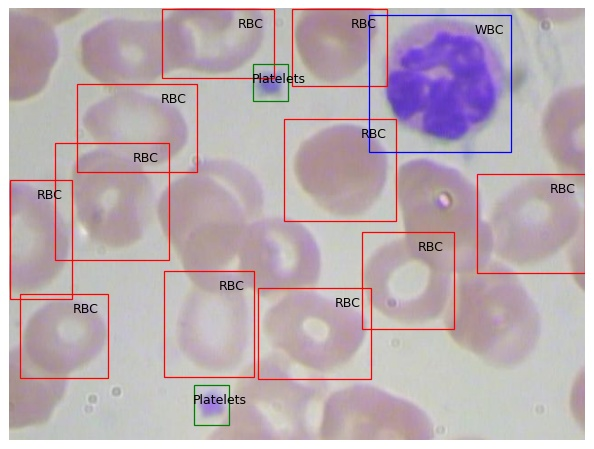
\includegraphics[width=0.40\textwidth]{img/rbc.jpg}
    \legend{Fonte: \cite{datasetBCCD}}
    \label{fig:fig1}
 \end{figure}
 
\subsubsection{Glóbulos Brancos}
Os glóbulos brancos, também conhecidos como \emph{White Blood Cells (WBC)}, são as células brancas do sangue, sendo responsáveis pela defesa do organismo contra as principais ameaças do corpo humano presentes no sistema sanguíneo. Através da fagocitose, que é um processo de englobamento de partículas sólidas pelas células, é realizado ações de defesa contra a invasão de fragmentos estranhos. Os glóbulos brancos são criados na medula óssea e estão presentes em todo o sangue, também em grande quantidade.

Se faz necessário a classificação dos diferentes tipos de células brancas e de suas importâncias para o sistema de defesa do organismo. É importante frisar que essa classificação se refere aos leucócitos maduros, mas também se pode encontrar presente os leucócitos imaturos (promielócitos, mielócitos, metamielócitos).

\begin{figure}[!htb]
    \centering
    \caption{Glóbulos Brancos (WBC)}
    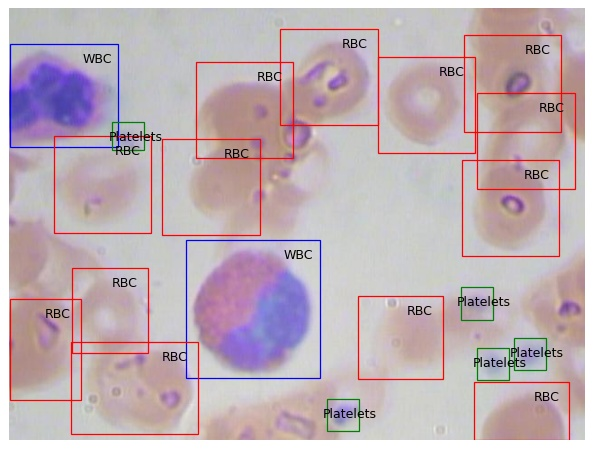
\includegraphics[width=0.40\textwidth]{img/wbc.jpg}
    \legend{Fonte: \cite{datasetBCCD}}
    \label{fig:fig2}
 \end{figure}
 
\begin{itemize}
    \item \textbf{Neutrófilos}: células brancas mais abundantes capazes de entrar nos tecidos, onde conseguem realizar a defesa do organismo, fagocitando partículas estranhas. Essas células são conhecidas como neutrófilos segmentados, pois existe uma célula percursora, que é o bastão, ou também chamado de neutrófilos bastonetes, que possuem essa nomenclatura pois seu núcleo não está amadurecido, ou seja ainda são jovens, e geralmente são identificados quando há infecções em fase aguda. 
    \item \textbf{Eosinófilos}: células brancas responsáveis na defesa contra parasitas, geralmente estão presentes em grande quantidade no sangue durante reações alérgicas e infestações parasitárias.
    \item \textbf{Basófilos}: células brancas atuantes em respostas alérgicas e na coagulação do sangue. São capazes de liberar histamina, contribuindo para respostas alérgicas ao dilatar e permeabilizar os vasos sanguíneos e também liberam heparina que é capaz de prevenir a coagulação do sangue.
    \item \textbf{Monócitos}: células brancas capazes de entrar no tecido conjuntivo frouxo, onde conseguem se desenvolver em grandes células com grande efeito fagocítico denominadas macrófagos, de forma a ingerir partículas estranhas ao organismo.
    \item \textbf{Linfócitos}: segundo tipo de célula branca mais abundante, são responsáveis e de extrema importância nas respostas imunes específicas do corpo humano, inclusive na produção de anticorpos.
\end{itemize}

\subsubsection{Plaquetas}
As plaquetas, também conhecidas e citadas como \emph{Platelets}, são os menores componentes do sangue e possuem grande responsabilidade na hemostasia, que é uma resposta fisiológica para a prevenção e interrupção de sangramentos e hemorragias, ou seja, elas atuam na manutenção dos vasos sanguíneos. As plaquetas são fragmentos do citoplasma de megacariócitos, ou seja, elas são produzidas na medula óssea como parte dessas células especializadas que irão se dividir posteriormente e gerar um grande número de plaquetas. Aproximadamente, para cada 1 megacariócito, se pode produzir cerca de 4000 plaquetas.

Devido ao fato de serem fragmentos de uma célula, as plaquetas não possuem núcleo e são muito pequenas, com aproximadamente de 1–3 µm de diâmetro, com a coloração azul-acinzentado. A vida útil das plaquetas dura em média de 9 a 12 dias, e elas são removidas pelo baço quando estão velhas ou danificadas.

\begin{figure}[!htb]
    \centering
    \caption{Plaquetas (Platelets)}
    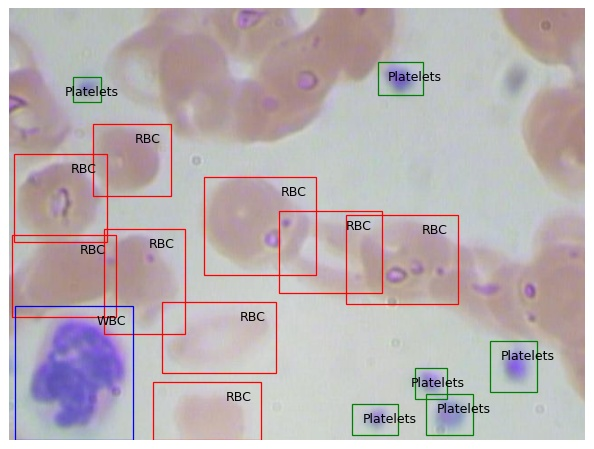
\includegraphics[width=0.40\textwidth]{img/plt.jpg}
    \legend{Fonte: \cite{datasetBCCD}}
    \label{fig:exemplo3}
 \end{figure}
 
\subsection{Hemograma}
Um hemograma, também conhecido e citado como \emph{Complete Blood Count (CBC)}, é um exame bastante comum e muito utilizado, onde se realiza uma análise de sangue que envolve a contagem das diferentes células sanguíneas. A partir dos números obtidos através dessa contagem e com a comparação desse valor com as faixas de normalidade, é possível chegar a diversas conclusões sobre a saúde do paciente e até mesmo já identificar alguma doença ou problema.

Um hemograma geralmente é realizado em duas principais etapas, sendo a primeira relacionada ao eritrograma que se refere à análise das células vermelhas, de forma a revelar até mesmo alguns tipos essenciais de alterações patológicas do sistema eritropoético, que é o sistema responsável pela produção do material vermelho do sangue, como aumento na produção de glóbulos vermelhos e anemias. A segunda parte está relacionada com o leucograma, que corresponde à contagem global e específica dos leucócitos, a parte branca do sangue. O quadro leucocitário resultante com o exame hematológico, possibilita ao médico tirar importantes conclusões.

\subsubsection{Eritrograma}
O objetivo do eritrograma ao realizar a análise da parte vermelha do sangue, é analisar alguns atributos chave, primeiramente é realizado a contagem geral dos eritrócitos adotando uma escala de milhões/mm³. A hemoglobina também será calculada e registrada em uma escala de g/dl.

Depois dessa principal contagem é calculado alguns índices importantes, sendo o primeiro deles o cálculo do volume corpuscular médio (VCM), que é o volume médio das hemácias, calculado pelo quociente de um determinado volume de hemácias pelo número de células contidas no mesmo volume. Outro importante atributo é a hemoglobina corpuscular média (HCM), que semelhante ao VCM, é o conteúdo médio da hemoglobina, calculado pelo quociente de conteúdo de hemoglobina em um determinado volume de hemácias pelo número de células contidas no mesmo volume.

Também temos outro índice que é a concentração de hemoglobina corpuscular média (CHCM), sendo a percentagem da hemoglobina em uma amostra de 100ml de hemácias. Por fim temos, a amplitude de distribuição dos glóbulos vermelhos, que em inglês significa \emph{Red Cell Distribution Width (RDW)}, que será responsável por avaliar a variação de tamanho entre as hemácias.

\subsubsection{Leucograma}
O objetivo do leucograma ao realizar a análise da parte branca do sangue, assim como no eritrograma, é analisar alguns atributos chave, porém diferente do processo anterior, essa etapa terá um foco muito maior na classificação e contagem de diferentes células brancas.

Primeiramente é feita uma contagem geral de leucócitos em mm³. Depois é realizada a contagem de forma a classificar cada tipo de leucócito presente, com neutrófilos, eosinófilos, basófilos, linfócitos, monócitos e também os granulócitos imaturos (promielócitos, mielócitos, metamielócitos). Por fim, também é calculado o número presente de plaquetas no sangue em mm³.

\section{Deep Learning}
\label{sec:conceito2}

\chapter{Estado da Arte da Área Pesquisada}
\label{chap:mapeamento}

O processo de pesquisa e seleção dos trabalhos relacionados, foi realizado com base em um mapeamento sistemático sobre as pesquisas com propostas para agilizar a identificação e interpretação de análises de sangue. Esta revisão resultou na identificação e seleção dos principais trabalhos de pesquisa no tema deste Projeto de Trabalho de Conclusão de Curso. Outro objetivo deste mapeamento sistemático foi verificar os métodos utilizados para a aplicação de Deep Learning em imagens de sangue em placas de petri de maneira que possam ser aplicados neste projeto de forma satisfatória.

\section{Mapeamento Sistemático da Literatura}

O mapeamento sistemático da literatura é realizado com base na busca e levantamento de artigos, para isso se utiliza uma string de busca para as principais bibliotecas e repositórios de artigos. Esses artigos serão analisados e selecionados conforme a sua área de pesquisa e a sua temática, para inclusão nesse estudo. Para isso, se é utilizado uma ferramenta para automatização dessa tarefa, que é o Parsifal\footnote[1]{https://parsif.al/}, de modo a definir a string de busca, salvar os artigos necessários e realizar a seleção.

As questões de pesquisas levantadas para isso foram, ``Como os algoritmos de Deep Learning podem ser utilizados para a interpretação de exames?'' e ``Como realizar o tratamento de imagens para reconhecimento por modelos de Deep Learning?''. A partir dessas questões se foram extraídas palavras e termos para o direcionamento da pesquisa. Podemos visualizar estas palavras com seus sinônimos na Tabela 1.

\begin{center}
Tabela 1 - Tabela com Palavras-Chave e Sinônimos
\begin{center}
\begin{tabular}{|c|c|}
\hline
\textbf{Palavra-Chave} & \textbf{Sinônimos} \\ \hline
Blood Analysis & Blood Sample \\ \hline
Classification & Interpretation, Recognition \\ \hline
Deep Learning & Artificial Intelligence, Computer Vision, Machine Learning \\ \hline
\end{tabular}
\end{center}
Fonte: Elaborada pelo Autor
\end{center}

Na Tabela 2, é listado as bases de dados onde os artigos foram coletados, a quantidade de cada um de les e a string de busca utilizada na seleção. A mesma string de busca foi utilizado nas três bases de dados, e os artigos encontrados foram dos últimos 5 anos.

\clearpage
\begin{center}
Tabela 2 - Bases de Dados e Quantidade de Artigos Selecionados
\begin{center}
\begin{tabular}{|c|c|c|}
\hline
\textbf{Base de Dados} & \textbf{Artigos} & \textbf{String de Busca} \\ \hline
\multirow{2}{*}{ACM Digital Library} & \multirow{2}{*}{37} & \multirow{6}{*}{\begin{tabular}[c]{@{}c@{}}(``classification'' OR ``interpretation'' OR ``recognition'') AND\\  (``deep learning'' OR ``artificial intelligence'' \\ OR ``computer vision'' OR ``machine learning'') AND\\  (``blood analysis'' OR ``blood sample'')\end{tabular}} \\
 &  &  \\ \cline{1-2}
\multirow{2}{*}{IEEE Digital Library} & \multirow{2}{*}{13} &  \\
 &  &  \\ \cline{1-2}
\multirow{2}{*}{Scopus} & \multirow{2}{*}{114} &  \\
 &  &  \\ \hline
\end{tabular}
\end{center}
Fonte: Elaborada pelo Autor
\end{center}

\subsection{Critérios de Exclusão}

Os artigos coletados na pesquisa através da string de busca, passaram por critérios de exclusão por não se adequarem a esta pesquisa, esses critérios podem ser observados na Tabela 3. 

\begin{center}
Tabela 3 - Critérios de Exclusão
\begin{center}
\begin{tabular}{|c|c|}
\hline
\textbf{Critério de Exclusão} & \textbf{Nº de Artigos Recusados} \\ \hline
O estudo não faz parte da área de pesquisa & 101 \\ \hline
O estudo apresenta resultados fora da computação & 29 \\ \hline
O estudo não é um estudo primário & 6 \\ \hline
O estudo é duplicado & 16 \\ \hline
\end{tabular}
\end{center}
Fonte: Elaborada pelo Autor
\end{center}

A seleção inciou com 164 artigos no total das três bases de dados buscadas. Com a aplicação dos critérios de exclusão, observa-se um resultante de apenas 14 artigos. Isso ocorreu pois 101 artigos foram eliminados no critério ``O estudo não faz parte da área de pesquisa'', que significa que esses artigos tinham alguma relação, porém eram voltados a outras áreas. Outros 29 artigos foram eliminados no critério ``O estudo apresenta resultados fora da computação'', que significa que eram da área de pesquisa, porém com resultados e métodos sem conexão com a computação. Foram também encontrados 6 artigos, que entraram no critério ``O estudo não é um estudo primário'', o que indica que o artigo pode ser uma revisão sistemática da literatura ou semelhante. Por fim, foram eliminados outros 16 artigos por serem duplicados.

\subsection{Critérios de Inclusão}

Os seguintes critérios de inclusão foram definidos:
\begin{itemize}
\item Nova tecnologia para análise de sangue;
\item Processo, método ou técnica para contagem de células sanguíneas;
\item Sistema para elaboração de hemogramas utilizando Deep Learning;
\end{itemize}

Na tabela 4, podemos encontrar todos os 14 artigos selecionados com base nos critérios de inclusão, todos eles se enquadram em pelo menos um deles.

\begin{center}
Tabela 4 - Artigos Selecionados
\begin{center}
\begin{tabular}{|c|l|l|}
\hline
\textbf{ID} & \multicolumn{1}{c|}{\textbf{Título do Artigo}} & \multicolumn{1}{c|}{\textbf{Autores}} \\ \hline
A1 & \begin{tabular}[c]{@{}l@{}}Analyzing microscopic images of \\ peripheral blood smear \\ using deep learning\end{tabular} & \begin{tabular}[c]{@{}l@{}}Mundhra, D. and Cheluvaraju, B. \\ and Rampure, J. and Rai Dastidar, T.\end{tabular} \\ \hline
A2 & \begin{tabular}[c]{@{}l@{}}Automatic detection and classification \\ of leukocytes using \\ convolutional neural networks\end{tabular} & \begin{tabular}[c]{@{}l@{}}Zhao, J. and Zhang, M. \\ and Zhou, Z. and Chu, J. and Cao, F.\end{tabular} \\ \hline
A3 & \begin{tabular}[c]{@{}l@{}}Automatic white blood cell classification \\ using pre-trained deep learning models: \\ ResNet and Inception\end{tabular} & \begin{tabular}[c]{@{}l@{}}Habibzadeh, M. and Jannesari, M. \\ and Rezaei, Z. and Baharvand, H. \\ and Totonchi, M.\end{tabular} \\ \hline
A4 & \begin{tabular}[c]{@{}l@{}}Classification of Human White \\ Blood Cells Using Machine Learning \\ for Stain-Free Imaging \\ Flow Cytometry\end{tabular} & \begin{tabular}[c]{@{}l@{}}Lippeveld, M. and Knill, C. and \\ Ladlow, E. and \\ Fuller, A. and Michaelis, L.J. and \\ Saeys, Y. and Filby, A. and Peralta, D.\end{tabular} \\ \hline
A5 & \begin{tabular}[c]{@{}l@{}}Blood cell classification using the hough\\ transform and \\ convolutional neural networks\end{tabular} & \begin{tabular}[c]{@{}l@{}}Molina-Cabello, M.A. and López-Rubio, E. \\ and Luque-Baena, R.M. and \\ Rodríguez-Espinosa, M.J. and \\ Thurnhofer-Hemsi, K.\end{tabular} \\ \hline
A6 & \begin{tabular}[c]{@{}l@{}}White Blood Cells Image Classification \\ Using Deep Learning with \\ Canonical Correlation Analysis\end{tabular} & Patil, A.M. and Patil, M.D. and Birajdar, G.K. \\ \hline
A7 & \begin{tabular}[c]{@{}l@{}}Image processing and machine learning\\ in the morphological analysis \\ of blood cells\end{tabular} & \begin{tabular}[c]{@{}l@{}}Rodellar, J. and Alférez, S. and Acevedo, A. \\ and Molina, A. and Merino, A.\end{tabular} \\ \hline
A8 & \begin{tabular}[c]{@{}l@{}}Improving blood cells classification in \\ peripheral blood smears using \\ enhanced incremental training\end{tabular} & Al-qudah, R. and Suen, C.Y. \\ \hline
A9 & \begin{tabular}[c]{@{}l@{}}Corruption-Robust Enhancement of \\ Deep Neural Networks\\ for Classification of Peripheral \\ Blood Smear Images\end{tabular} & \begin{tabular}[c]{@{}l@{}}Zhang, S. and Ni, Q. and Li, B. and \\ Jiang, S. and \\ Cai, W. and Chen, H. and Luo, L.\end{tabular} \\ \hline
A10 & \begin{tabular}[c]{@{}l@{}}Convolutional neural network and decision \\ support in medical imaging:\\ Case study of the recognition of \\ blood cell subtypes\end{tabular} & Diouf, D. and Seck, D. and Diop, M. and Ba, A. \\ \hline
A11 & \begin{tabular}[c]{@{}l@{}}Combining Convolutional Neural Network\\ With Recursive Neural Network \\ for Blood Cell Image Classification\end{tabular} & \begin{tabular}[c]{@{}l@{}}Liang, G. and Hong, H. and Xie, W. and\\ Zheng, L.\end{tabular} \\ \hline
A12 & \begin{tabular}[c]{@{}l@{}}Blood diseases detection using \\ classical machine learning algorithms\end{tabular} & Alsheref, F.K. and Gomaa, W.H. \\ \hline
\end{tabular}
\end{center}
Fonte: Elaborada pelo Autor
\end{center}

Todos os artigos selecionados estão relacionados à maneiras e recursos para auxiliar na interpretação de exames de sangue utilizando conceitos de Deep Learning e Machine Learning.

\section{Análise dos trabalhos selecionados}

Por fim, com os artigos selecionados e classificados, é necessário realizar a extração dos dados desses trabalhos, sendo essa a última etapa desse mapeamento sistemático da literatura. É possível perceber que os algoritmos e abordagens mais utilizados são técnicas de \emph{Deep Learning}, como por exemplo, o uso de \emph{Convolutional Neural Network (CNN)} (A1, A2, A3, A4, A5, A6, A8, A9, A10, A11) e de \emph{Recurrent Neural Network (RNN)} (A6, A11), que são abordagens de redes neurais para a classificação das células sanguíneas.

Outros trabalhos utilizam de algoritmos de \emph{Machine Learning} tradicionais para a classificação, como por exemplo, ocorre com o uso de \emph{Random Forest} ou \emph{Decision Trees}  (A2, A4, A7), que são estruturas de árvores de decisão. Também se encontra estudos fazendo uso de \emph{Support Vector Machine (SVM)} (A7) que utilizam vetores de suporte e por fim \emph{K-Means e K-Nearest Neighbors (KNN)} (A12), que faz a classificação levando em conta os vizinhos mais próximos.

\chapter{Procedimentos Metodológicos}
\label{chap:metodologia}

\section{Recursos}

\chapter{Cronograma}
\label{chap:cronograma}

A Tabela \ref{tbl:cronograma} apresenta o cronograma de atividades propostas para o desenvolvimento deste projeto de trabalho de conclusão de curso, de forma a viabilizar <Falar sobre o que se pretende atingir com o projeto>.

\begin{table}[!htb]
\centering
\caption{Cronograma das atividades previstas.}
\label{tbl:cronograma}
\begin{tabular}{|l|c|c|c|c|c|c|c|c|c|c|}
\hline
\multicolumn{1}{|c|}{\textbf{Etapa}}       & \multicolumn{10}{c|}{\textbf{Meses}}                                                                                                                        \\ \hline
                                           & Fev & Mar & Abr & Mai & Jun & Ago & Set & Out & Nov & Dez \\ \hline
Fundamentação Teórica                      & X            & X            &              &              &              &                &                   &               &              &              \\ \hline
\makecell[l]{Mapeamento Sistemático \\ da Literatura}       &              &              & X            & X            &              &                &                   &               &              &              \\ \hline
\makecell[l]{Escrita do Projeto de TCC \\ e Defesa}         &              &              & X            & X            & X            &                &                   &               &              &              \\ \hline
\makecell[l]{Atividade a ser desenvolvida 1}              &              &              &              &              &              & X              &                   &               &              &              \\ \hline
\makecell[l]{Atividade a ser desenvolvida 2}             &              &              &              &              &              &                & X                 &               &              &              \\ \hline
\makecell[l]{Atividade a ser desenvolvida 3} &              &              &              &              &              &                & X                 & X             &              &              \\ \hline
\makecell[l]{Verificação de Aceitação dos \\ Resultados}    &              &              &              &              &              &                &                   & X             &              &              \\ \hline
\makecell[l]{Comparação dos Resultados \\ com a Literatura} &              &              &              &              &              &                &                   & X             & X            &              \\ \hline
Exposição dos Resultados                   &              &              &              &              &              &                &                   &               & X            &              \\ \hline
Escrita do TCC                             &              &              &              &              &              &                &                   &               & X            & X            \\ \hline
Defesa do TCC                              &              &              &              &              &              &                &                   &               &              & X            \\ \hline
\end{tabular}
\vspace{6pt}
\legend{Fonte: Elaborada pelo autor.}
\end{table}

As atividades propostas neste cronograma podem sofrer leves alterações no decorrer do seu desenvolvimento de acordo com a necessidade.

A forma mais fácil de criar tabelas é através de ferramentas gráficas. Geralmente utiliza-se o site \url{https://www.tablesgenerator.com/} para realizar tal atividade, exportando o código LaTeX e colando na parte do texto que ela deve aparecer~\cite{tablegenerator2021}.